\section{Benutzungsoberfl"ache}

%\comment{Was sind die grundlegenden Anforderungen an die Benutzungsoberfl"ache (Bildschirmlayout, Dialogstruktur, ...)?}
\begin{description}
	Das Modul ist in drei Container gegliedert. Der Inhalt der beiden gro"sen Container ist mithilfe eines Drop-Down-Men"us frei w"ahlbar.
	Die einzelnen Inhalte werden im Folgenden als Widget bezeichnet.
\end{description}

\subsection{Entwurf}
\begin{center}
	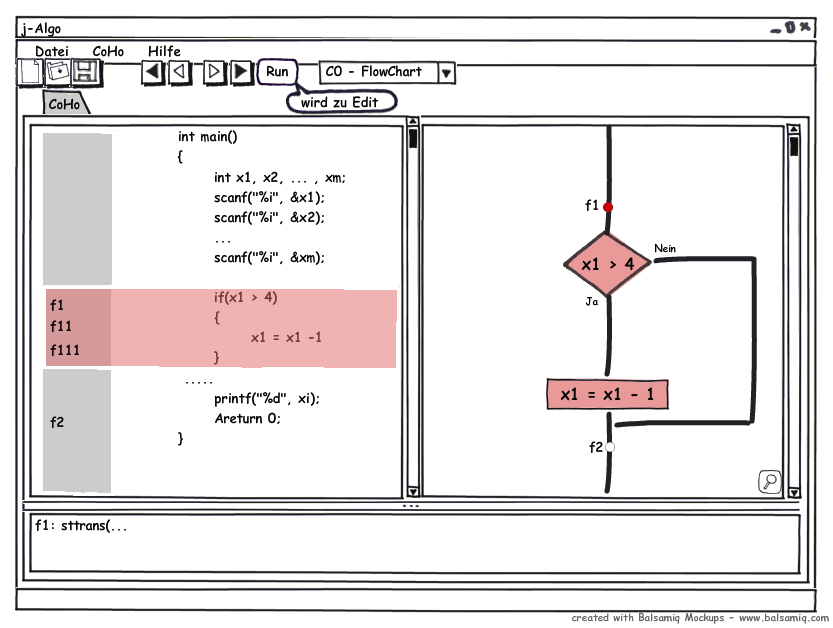
\includegraphics[scale=0.50]{images/Mockup_xml_design.png}
%	\captionof{figure}{Mockup}
\end{center}


\subsection{Workflow}
	\begin{enumerate}
		\item Willkommens-Ansicht
		\begin{description}
			Die erste Ansicht enth"alt den $C_0$-Editor im linken, sowie die Optionen im rechten Container.
			Der Benutzer w"ahlt  zuerst eine der Optionen aus dem Widget rechts aus und gelangt dann in den Editor-Modus.
		\end{description}

		\item Editor-Modus
		\begin{description}
			Hier steht einem nur das $C_0$-Code Widget zu Verf"ugung.
			Bei Bet"atigung des Run-Buttons wird der Code evaluiert und es wird gegebenenfalls in den Umwandlungs-Modus gewechselt.
		\end{description}

		\item Umwandlungs-Modus
		\begin{description}
			Im Umwandlungs-Modus ist der $C_0$-Code nicht mehr editierbar.
			Der Code kann schrittweise oder auch sofort vollst"andig durchlaufen werden, wobei er entsprechend
			in ein Flussdiagramm bzw. in $H_0$-Code umgewandelt wird.
			Ebenso ist es m"oglich, das Flussdiagramm in $H_0$-Code umzuwandeln.
		\end{description}
	\end{enumerate}
	


\subsection{Widgets}
	\subsubsection{Optionen}
		Dieser Teil orientiert sich optisch an anderen j-Algo-Modulen (z. B. KMP, AVL oder Hoare), 
		ist allerdings nur in der rechten H"alfte eingeblendet und bietet folgende Optionen:
		\begin{enumerate}
			\item "Offnen von $C_0$-Dateien
			\item "Offnen von Lehrbeispielen
			\item Eingabe der m-k-i-Parameter f"ur den $C_0$-Code
		\end{enumerate}

	\subsubsection{$C_0$-Editor}
		\begin{description}
			Dieser ist im Editor-Modus ein reiner Texteditor.
			Im Umwandlungs-Modus wird der Code formatiert und die Textbl"ocke werden semantisch hervorgehoben.
			Zus"atzlich werden baumstrukturierte Adressen angezeigt.
			Durch Anklicken werden korrespondierende Stellen in anderen Widgets hervorgehoben.
		\end{description}

	\subsubsection{Flussdiagramm}
		\begin{description}
			Dieses entspringt dem Beispiel aus dem Skript.
			Die baumstrukturierten Adressen werden an Knotenpunkten eingeblendet.
			Durch Anklicken werden korrespondierende Stellen in anderen Widgets hervorgehoben.
		\end{description}

	\subsubsection{$H_0$-Ansicht}
		\begin{description}
			Diese enth"alt den generierten $H_0$-Code.
			Durch Anklicken werden korrespondierende Stellen in anderen Widgets hervorgehoben.
		\end{description}	

	\subsubsection{Transformationsschritte}
		\begin{description}
			Hier werden die im Skript erw"ahnten "Ubersetzungsregeln bei Ausf"uhrung dargestellt.
		\end{description}

